\begin{surferPage}{An $A_3^{--}$ Singularity}
By looking the equation 
    \[x^4-y^2-z^2=0\]
    we can see that this surface is very similar to the preceeding one (an
    $A_3^{+-}$ with equation $x^4+y^2-z^2$).
    The leftmost picture below visualizes this by showing both surfaces in one
    picture ($A_3^{--}$ in yellow, $A_3^{+-}$ in blue).
    Cutting both surfaces with the plane $y=0$ we get the same curve in both
    cases: 
    \vspace*{-0.5em}
    \begin{center}
      \begin{tabular}{c@{\qquad}c}
        \begin{tabular}{@{}c@{}}
          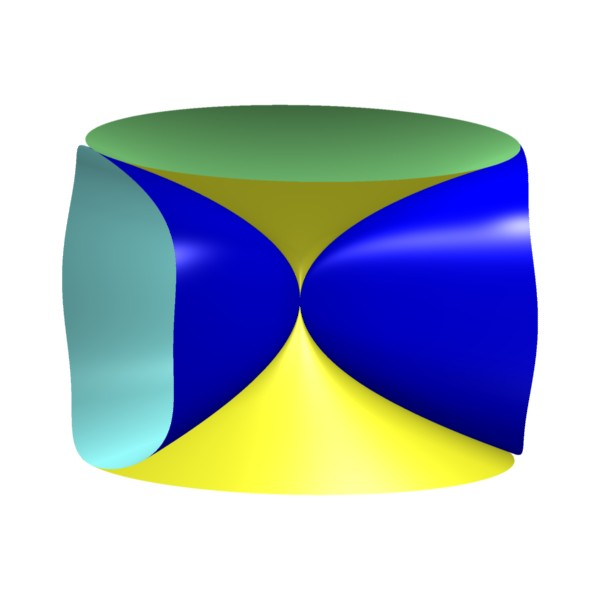
\includegraphics[width=1.6cm]{../../common/images/A3pmA3mm}
        \end{tabular}
        &
        \begin{tabular}{@{}c@{}}
          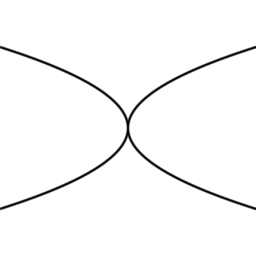
\includegraphics[width=1.6cm]{../../common/images/A3pm_cut}
        \end{tabular}
      \end{tabular}
    \end{center}
    \vspace*{-0.1cm}
    We my deform this $A_k$-singularity into $\lfloor\frac{k+1}{2}\rfloor$
    double cones, too:
%    \dontshow{
    % 
    \begin{center}
      \vspace*{-0.1cm}
      \begin{tabular}{@{}c@{\quad}c@{\quad}c@{}}
        \begin{tabular}{@{}c@{}}
          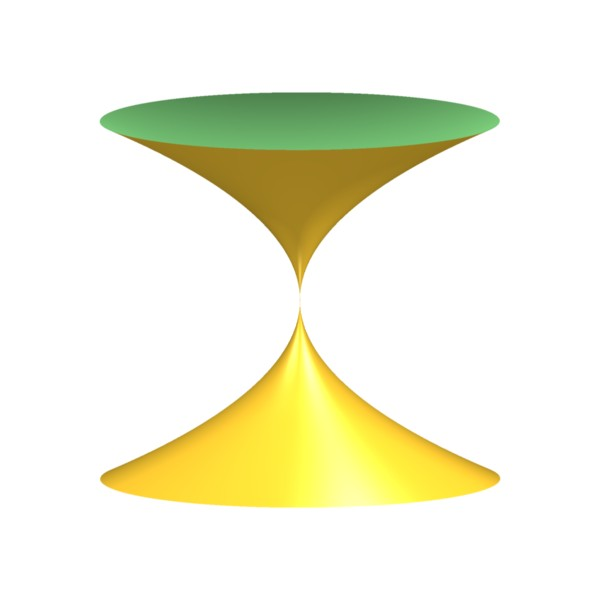
\includegraphics[width=1.6cm]{../../common/images/A3mm_0}
        \end{tabular}
        &
        \begin{tabular}{@{}c@{}}
          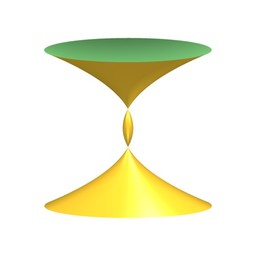
\includegraphics[width=1.6cm]{../../common/images/A3mm_1}
        \end{tabular}
        &
        \begin{tabular}{@{}c@{}}
          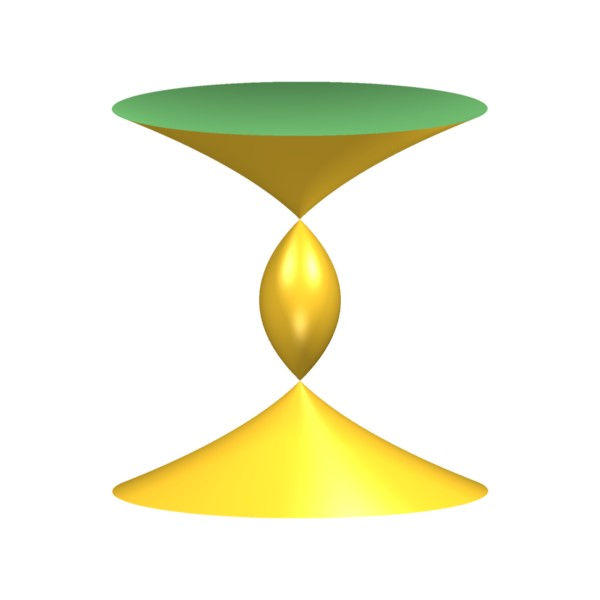
\includegraphics[width=1.6cm]{../../common/images/A3mm_2}
        \end{tabular}
      \end{tabular}
    \end{center}
%    }
    \vspace*{-0.2cm}
    We can realize the deformation of the $A_3^{--}$ singularity shown above
    with the following formula:
    \[\bigl(x-\frac12 a^2\bigr)^2\bigl(x+\frac12 a^2\bigr)^2-y^2-z^2.\]
 
\end{surferPage}
